% Пример статьи для журнала КИО
\documentclass[intlimits,twoside,a4paper,11pt]{article}

% текст статьи рекомендуется писать в кодировке utf-8
\usepackage[utf8]{inputenc}

% Подключение пакета с шаблоном журнала.
% Необзятальная опция eqsecnum указывает, что в каждом разделе формулы нумеруются заново.
\usepackage[eqsecnum]{kioj2}
% Здесь можно подключить свои пакеты. Некоторые пакеты работают только если их подключить перед предыдущей строкой \usepackage[eqsecnum]{kioj2}
% \usepackage[•]{•}
\usepackage{array}

% Указываем номер страницы, с которой начинается статья, можно не указывать, будет нумероваться с первой.
\setcounter{page}{42}

%рубрика в журнале, обычно не известна при подаче статьи, поэтому не указываем
\journalsectionnoimage{}
%\journalsection{informatics}
%\journalsection{information-systems}
%\journalsection{software-engineering}
%\journalsection{computer-in-education}
%\journalsection{popular-science-articles}
%\journalsection{programming-practice}
%\journalsection{editorial-column}
%\journalsection{specialists-training-new-teaching-methods}
%\journalsection{specialists-training-training-programs}
%\journalsection{specialists-training-professional-standards}
%\journalsection{open-problems-for-young-scientists}
%\journalsection{empty}

%указывам год, номер выпуска неизвестен, поэтмоу ставим прочерк, указываем edu, что означает журнал "компьютерные инструменты в образовании".
\issue{2015}{-}{edu}
% Указываем УДК для статьи
\udknumber{621.320}
% Указываем DOI для статьи, можно не указывать
\doinumber{10.1000/182}

%Указываем название статьи в обычном регистре в квадратных скобках, потом заглавными буквами в фигурных скобках. Второй вариант будет использоваться только в заголовке, первый вариант будет использоваться во всех других местах, в частности, при цитировании.
\title[Название статьи]{НАЗВАНИЕ СТАТЬИ}

%Информация об авторах. Каждый автор указывается отдельно с помощью трех инструкций \authorI, \authorIaddr, \authorIemail. Номера авторов могут быть I, II, III, IV, V.
%в команде \author* указывается сначала имя автора с инициалами в квадратных скобках, потом указывается полное имя автора. Полное имя используется только при выводе расширенной информации об авторе.
%в команде \affil указывается через запятую список организаций, которые представляет автор. Сами организации указываются ниже командой \affiliation.
%\authorIaddr и \affilitaion различаются тем, что первое является кратким расском об авторе, в отличие от второго, где указывается только организация.
\authorI[Андреев А.~А.\affil{1,2}]{Андреев Андрей Андреевич}
\authorIaddr{звания, должность, организация}
\authorIemail{aaa@org.com}

\authorII[Борисов Б.~Б.\affil{2}]{Борисов Борис Борисович}
\authorIIaddr{д.ф.н., профессор кафедры философии ?ГУ,}
\authorIIemail{bbb@org.com}

\affiliation{1}{СПбГУ}
\affiliation{2}{СПбЭТУ}

\begin{document}
\maketitle

\begin{abstract}
Здесь пишется аннотация, на русском.
Здесь пишется аннотация, на русском.
Здесь пишется аннотация, на русском.
Здесь пишется аннотация, на русском.
Здесь пишется аннотация, на русском.
Здесь пишется аннотация, на русском.
Здесь пишется аннотация, на русском.
Здесь пишется аннотация, на русском.
\keywords здесь перечисляются ключевые слова, через запятую, все слова с маленькой буквы.
%Команда \autocitationexample автоматически генерирует пример цитирования статьи, либо можно самостоятельно написать цитирование с помощью команды \citationexample
\autocitationexample
%\citationexample Андреев А.~А., Борисов Б.~Б. Шаблон статьи для журнала КИО. Нигде не опубликовано
\acknowledgements Здесь можно вставить благодарности и ссылки на гранты.
\end{abstract}

\section{ВВЕДЕНИЕ}
Заголовки всех разделов пишутся заглавными буквами. Подразделы и меньше~--- в обычном регистре.

\section{ПЕРВЫЙ РАЗДЕЛ}
Пример текста раздела. Пример текста раздела. Пример текста раздела. Пример текста раздела. Пример текста раздела. Пример текста раздела.
\begin{itemize}
\item Пример перечисления.
\item Второй пункт.
\item Третий пункт.
\end{itemize}

Теперь пример нумерованного списка.
\begin{enumerate}
\item Первый пункт;
\item Второй пункт;
\item Третий пункт.
\end{enumerate}
Ссылка на рис.~\ref{fig-example}

\begin{figure}[htb]
\centering
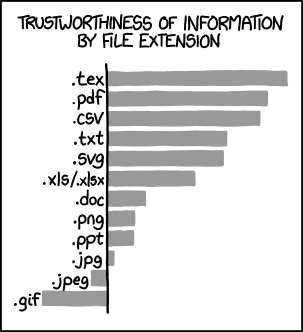
\includegraphics[width=0.4\textwidth]{xkcd1301.png}
\caption{Достоверность информации в зависимости от расширения файла} \label{fig-example}
\end{figure}

%Пример таблицы. [H] означает, что таблица должна быть ровно здесь и никуда не перемещаться.
\begin{table}[H]
\centering
\caption{Пример таблицы}
\label{table-example}
\small
\begin{tabular}{|p{5cm}|c|}
	\hline
	\centering
	Вопрос & ? \\
	\hline
	Ответ & 42 \\
	\hline
\end{tabular}
\end{table}

\subsection{Подраздел}
\label{sec:sub} %ссылка на раздел
Текст в подразделе

\subsubsection{Подподраздел}
Сначала, ссылка на \ref{sec:sub}.
%Текст в подподразделе с примером рисунка, состоящего из двух других рисунков. Мы можем ссылаться либо на рисунок полностью, например,~\ref{fig-example-2}, либо на подрисунки, например,~\ref{fig-example-2b}.

%Далее пример двух изображений рядом на одном рисунке
%Чтобы это работало, в начале файла нужно подключить пакет subcaption:
%\usepackage{subcaption}
\begin{figure}[H]
	\centering
	\begin{subfigure}[t]{70mm} %указываем размер подрисунка, без буквы [t] картинки будут вертикально отцентрованы
		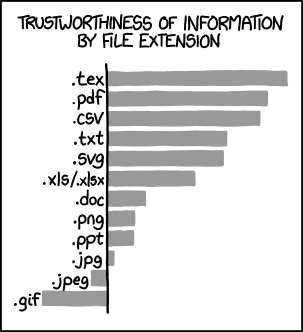
\includegraphics[width=\textwidth]{xkcd1301.png} %width=\textwidth указывает, что ширина совпадает с шириной подрисунка
		\subcaption{Необязательный подзаголовок}
		\label{fig-example-2a}
	\end{subfigure}
	\quad %это широкий пробел между двумя рисунками
	\begin{subfigure}[t]{50mm}
		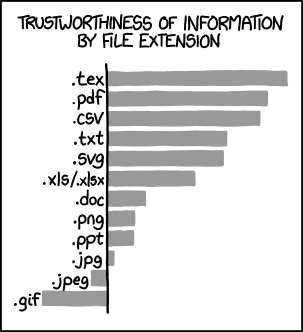
\includegraphics[width=\textwidth]{xkcd1301.png}
		\subcaption{} % Здесь подзаголовок не указан
		\label{fig-example-2b}
	\end{subfigure}
	\caption{Пример двух изображений рядом на одном рисунке} \label{fig-example-2}
\end{figure}

\section{ЗАКЛЮЧЕНИЕ}
Текст заключения с примером ссылки на литературу:~\cite{lib-1,lib-2}

%Оформляем литературу, 9 означает, что у нас не более 9 пунктов в списке, т.е. все номера состоят из не более, чем одной цифры. Если пунктов много, т.е. номера могут быть двузначными, пишем 99.
\begin{thebibliography}{9}
\bibitem{lib-1} {\it Madhav S.} Game Programming Algorithms and Techniques: A Platform-Agnostic Approach (Game Design). UK, 2013. 
\bibitem{lib-2} {\it Ericson C.} Real-Time Collision Detection. USA, 2004.
\end{thebibliography}

%дополнительная информация о статье
\additionalinfo{ГРНТИ 00000}
\additionalinfo{Поступила в редакцию 2 января 2014, окончательный вариант 24 января 2016 г.}

%указываем, что теперь начинается английская часть

\begin{translatedpart}
%указываем название и авторов на английском
\title{English title}
\authorI[Andreev A.~A.\affil{1,2}]{Andreev Andrey Andreevich}
\authorIaddr{position position position position position,
institution institution institution institution institution}

\authorII[Borisov B.~B.\affil{2}]{Borisov Boris Borisovich}
\authorIIaddr{just a cool guy with some position at some institution}

\affiliation{1}{SPbSU}
\affiliation{2}{SPbETU}

%даем команду на печать английского заголовка
\maketranslatedtitle

\begin{abstract}
English abstract goes here. English abstract goes here. English abstract goes here. English abstract goes here.
English abstract goes here. English abstract goes here. English abstract goes here. English abstract goes here.

English abstract goes here. English abstract goes here. English abstract goes here. English abstract goes here.
English abstract goes here. English abstract goes here. English abstract goes here. English abstract goes here.


English abstract goes here. English abstract goes here. English abstract goes here. English abstract goes here.
English abstract goes here. English abstract goes here. English abstract goes here. English abstract goes here.

English abstract goes here. English abstract goes here. English abstract goes here. English abstract goes here.
English abstract goes here. English abstract goes here. English abstract goes here. English abstract goes here.

\keywords keywords, separated by comma, in lower case.
\autocitationexample
%\citationexample ???
\acknowledgements here we may thank everybody who helped authors with this paper, and name grants that supported the research and the paper.
\end{abstract}

\additionalinfo{Received October 7, 2001, The final version: December 28, 2015}

\end{translatedpart}

%Завершаем статью печатью информации об авторах.
\makekioauthors

\end{document}
